The hardware for the Fido artificial intelligence was chosen using three main parameters.  Firstly, the electrical components had to support and compliment the software library; it would be impractical to refactor the entire code-base.  Secondly, the hardware had to be easily trainable and debuggable.  Lastly the sensors and design chosen had to facilitate the concept of natural learning, modeling after nature to some degree.

\subsection{Preliminary Decisions}

The Teensy 3.1 microcontroller development system was chosen as the host platform for Fido's hardware implementation.  As the board already has a USB bootloader and an open source software toolchain, it allowed for rapid prototyping of the hardware and software.  The core microcontroller of the Teensy sports an ARM 32 bit, 72 MHz Cortex-M4 architecture, giving Fido necessary computational power.  While a microcontroller with an integrated floating point unit may have sped up the numerous floating point multiplication operations involved in neural network propagation, it was decided unnecessary for this prototype due to time and cost considerations.

% wrap text around maybe?
\begin{figure}[ht]
	\centering
	\scalebox{.6}{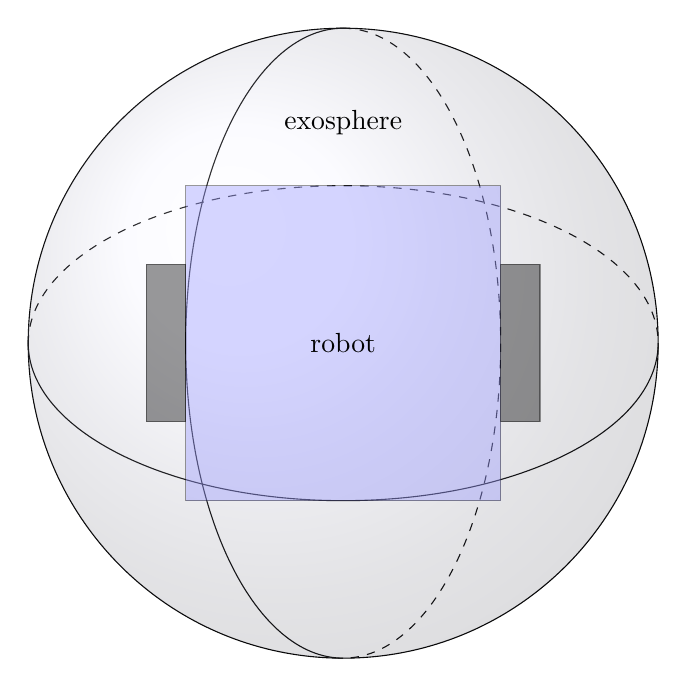
\begin{tikzpicture}
    \draw (-4,0) arc (180:360:4cm and 2cm);
    \draw[dashed] (-4,0) arc (180:0:4cm and 2cm);
    \draw (0,4) arc (90:270:2cm and 4cm);
    \draw[dashed] (0,4) arc (90:-90:2cm and 4cm);
    \draw (0,0) circle (4cm);
    \shade[ball color=blue!10!white,opacity=0.20] (0,0) circle (4cm);
    \fill[blue!40!white,draw=black,opacity=0.40] (-2,2) rectangle (2,-2);
    \fill[black,draw=black,opacity=0.40] (-2,1) rectangle (-2.5,-1);
    \fill[black,draw=black,opacity=0.40] (2,1) rectangle (2.5,-1);
    \node at (0,0) {robot};
    \node at (0,2.8) {exosphere};
\end{tikzpicture}}
	\caption{Differential Drive Robot in Exosphere}
\end{figure}

As Fido relies on inputs and outputs in order to learn and advance its neural networks, the selection of sensors and other peripherals was considered carefully.  The sensor outputs needed to be easily modified by a human for training to be feasible: an example is a light sensor being easier to control than a radiation or temperature sensor.  An obvious sensor choice was a microphone, allowing Fido to respond differently to sounds of various magnitude and frequency by passing in a sound wave.  Another sensor choice was infrared and visible light sensors.  While the choice of visible light may seem clear, infrared light was chosen as a one dimensional gradient input (the magnitude of the light) as something that could easily be applied and denied in a training environment.  Three dimensional acceleration, rotational velocity, and magnetic field sensors were also chosen to give Fido a sense of spatial awareness: through the accelerometer we could detect forces, through the gyroscope (measures rotational velocity) we could detect orientation, and through the magnetometer we could detect magnets (and the Earth's natural magnetic field).  Fido was also given the ability to detect it's own battery voltage to detect states of low and high charge, mimicking nature's state of tiredness.

Outputs were similarly chosen: motors allowed Fido to learn movement, a piezoelectric buzzer served as Fido's voice, and an RGB LED gave yet another output for easy training and debugging.  The drive system used by Fido for locomotion is a differential-drive arrangement placed inside of a large, hollow sphere.  Differential drive was chosen as a simple to understand kinematic model, while the reasoning for the exosphere was somewhat psychological: a ``hidden'' drive system gives a greater appearance of Fido learning how to move, as the potential for movement is obfuscated.  Additionally the exosphere provides protection against high bursts of acceleration used for training.

\subsection{Electrical Implementation}

\begin{figure}[ht]
	\centering
	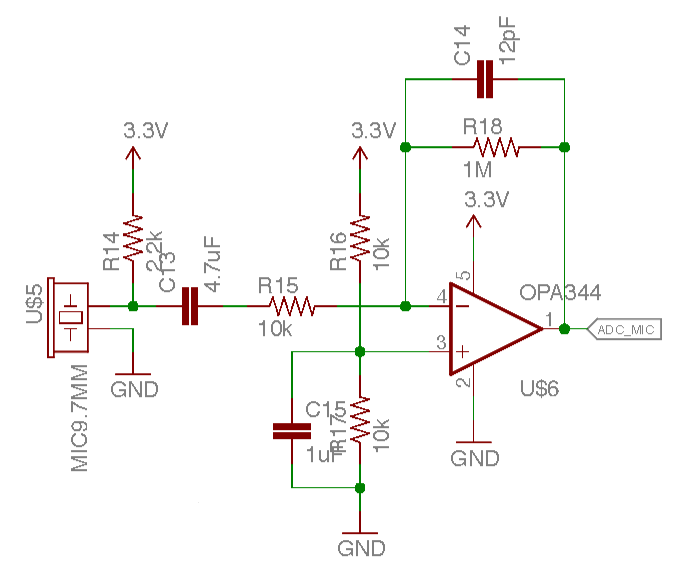
\includegraphics[height=5cm]{Figures/micDiagram.png}
	\caption{Schematic of Microphone Circuit}
\end{figure}

An electret microphone was chosen as a sound sensor to reduce much of complexity traditionally associated with microphones (mainly a polarizing power supply).  A simple amplifying circuit uses an OPA344 operational amplifier to increase millivolt level voltages to 3.3 volt levels readable by the Teensy ADC (analog to digital converter).

\begin{figure}[ht]
	\centering
	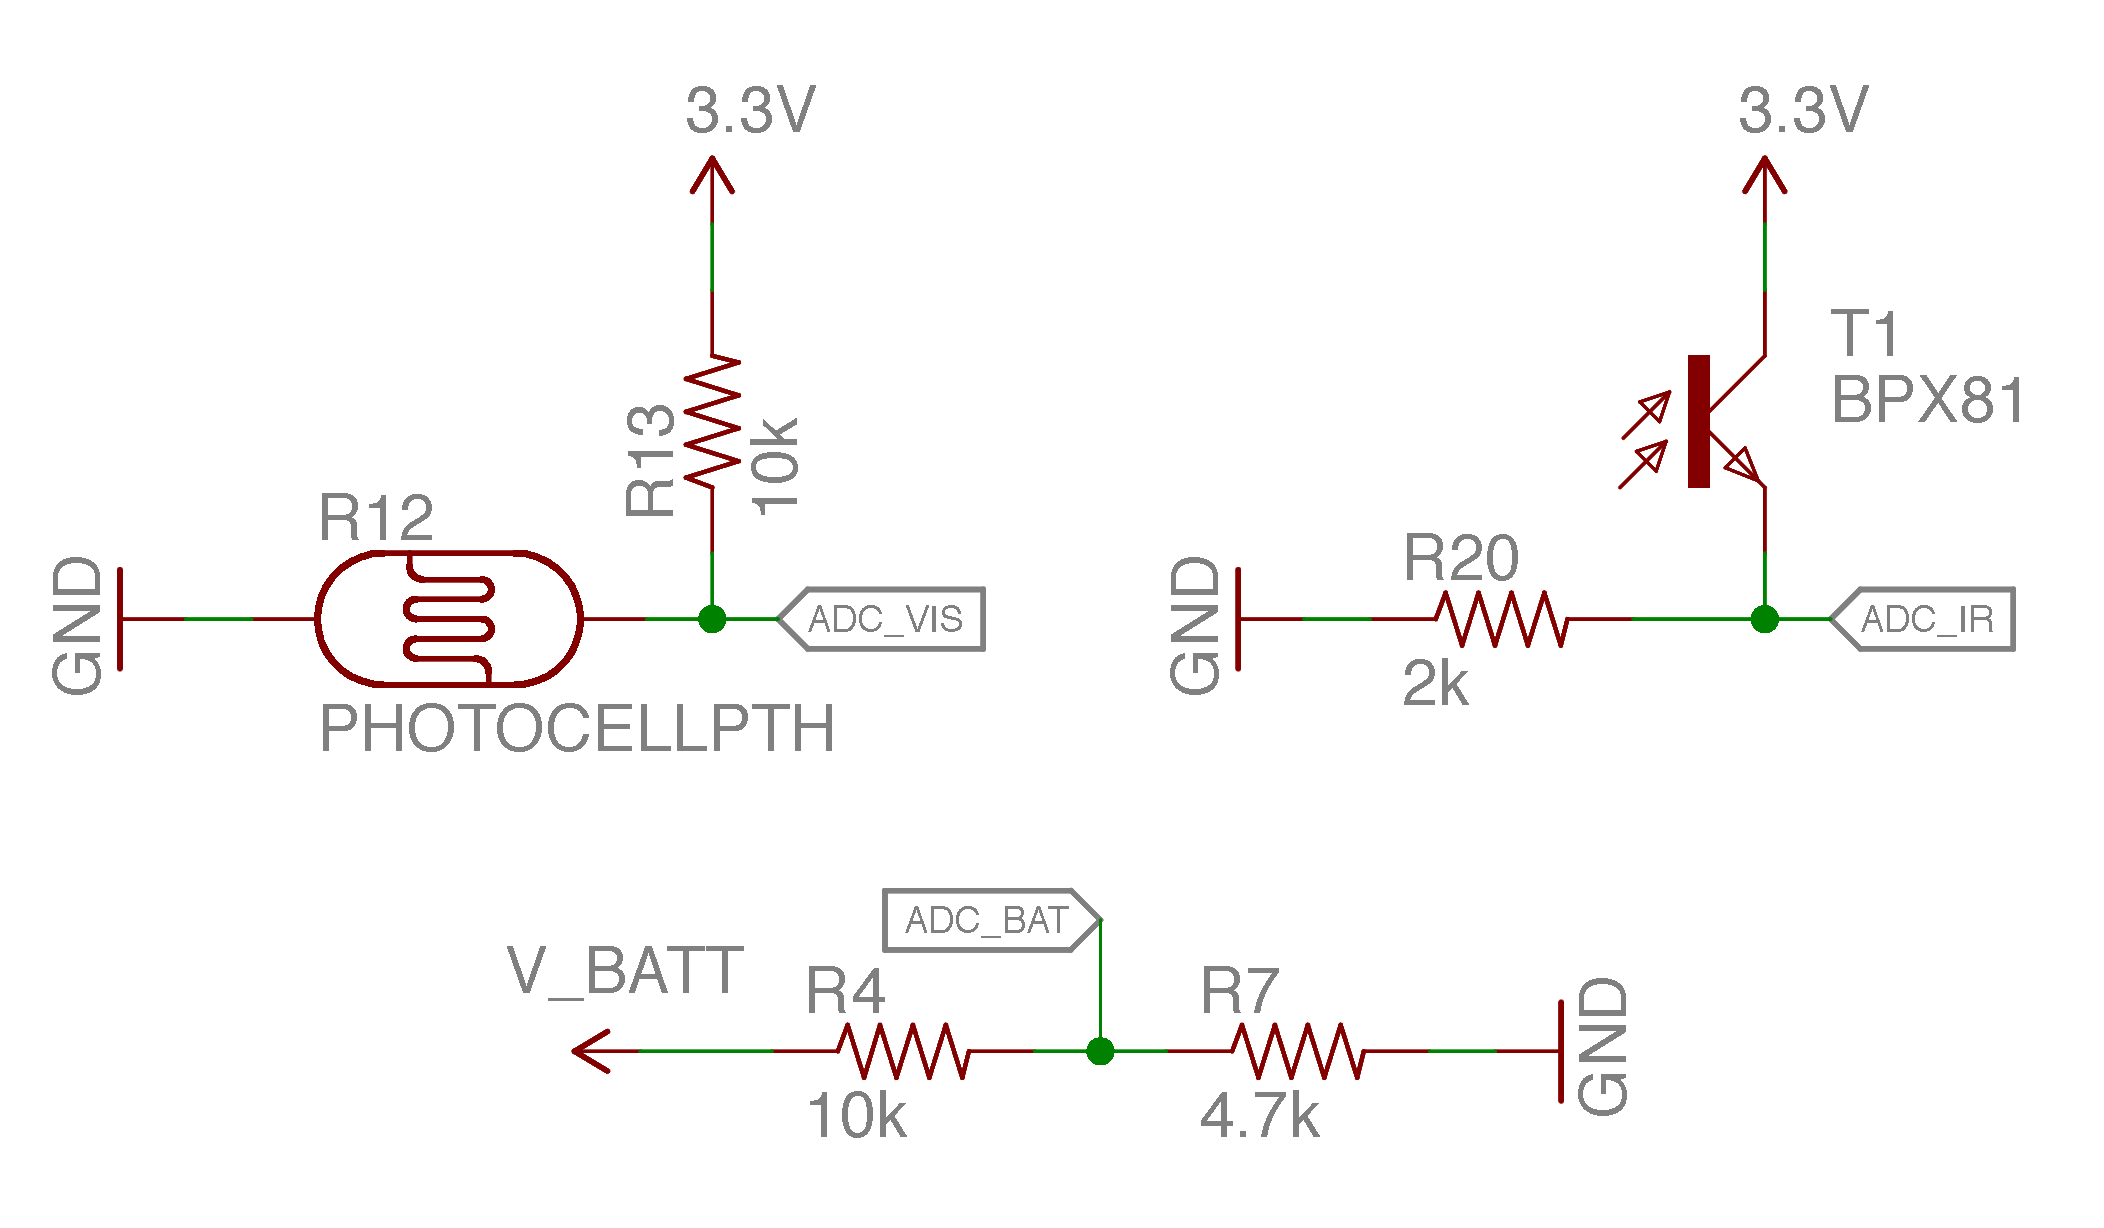
\includegraphics[height=5cm]{Figures/divDiagram.png}
	\caption{Analog Sensor Implementations}
\end{figure}

Visible light, infrared light, and battery level sensors were implemented using traditional voltage dividers: the ratio of $R_2$ to $R_1 + R_2$ determined the multiplier to the input voltage.  This makes the output voltage directly proportional to the change in one of the sensor's resistance, allowing us to read and process values using the Teensy's ADC.  For visible light a CdS photoresistor was used as $R_1$.  For infrared light a phototransistor was used instead due to most photoresistors' light sensitivity peaking at ~650nm, still in the visible light range.

\begin{figure}[ht]
	\centering
	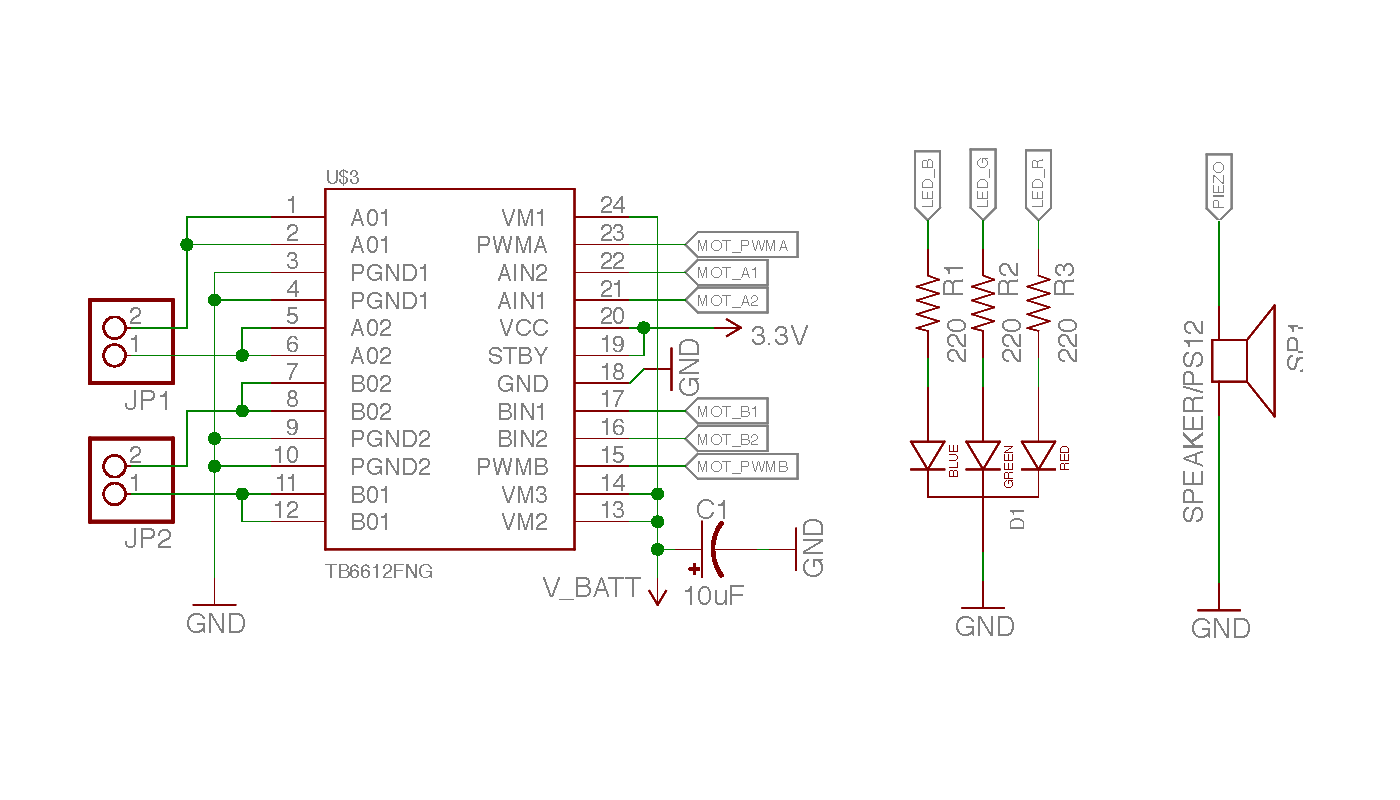
\includegraphics[height=5cm]{Figures/outDiagram.png}
	\caption{Fido Output Implementations}
\end{figure}

Fido's motor control was implemented using the TB6612FNG dual motor driver, chosen for its small SMD footprint and integrated flyback diodes to prevent back EMF.  When supply voltage is reduced across an inductive load such as a motor, there is often a voltage spike with the capability to damage sensitive electronics.  Integrated protection against this phenomenon made this driver a clear choice.  Additionally, the driver met current supply capabilities for the chosen DC brushed motors with a constant current of 1.2A per channel and a max current of 3.2A per channel.  An RGB LED was added with current limiting resistors to PWM (pulse width modulation) output channels on the Teensy, allowing variable brightness control.  A piezoelectric speaker was connected to the Teensy DAC (digital to analog converter) to facilitate clean audio generation.  In addition to the noted peripherals a MicroSD slot and Bluetooth 4.0 module were added for purposes of monitoring and debugging: Neural networks could be stored in text files on the MicroSD, while Fido could be connected to using a mobile application to configuration settings and select neural networks.  A complete schematic can be found in the Appendix of this paper.

\subsection{Mechanical Implementation and Fabrication}

% wrapped text def
\begin{figure}[ht]
	\centering
	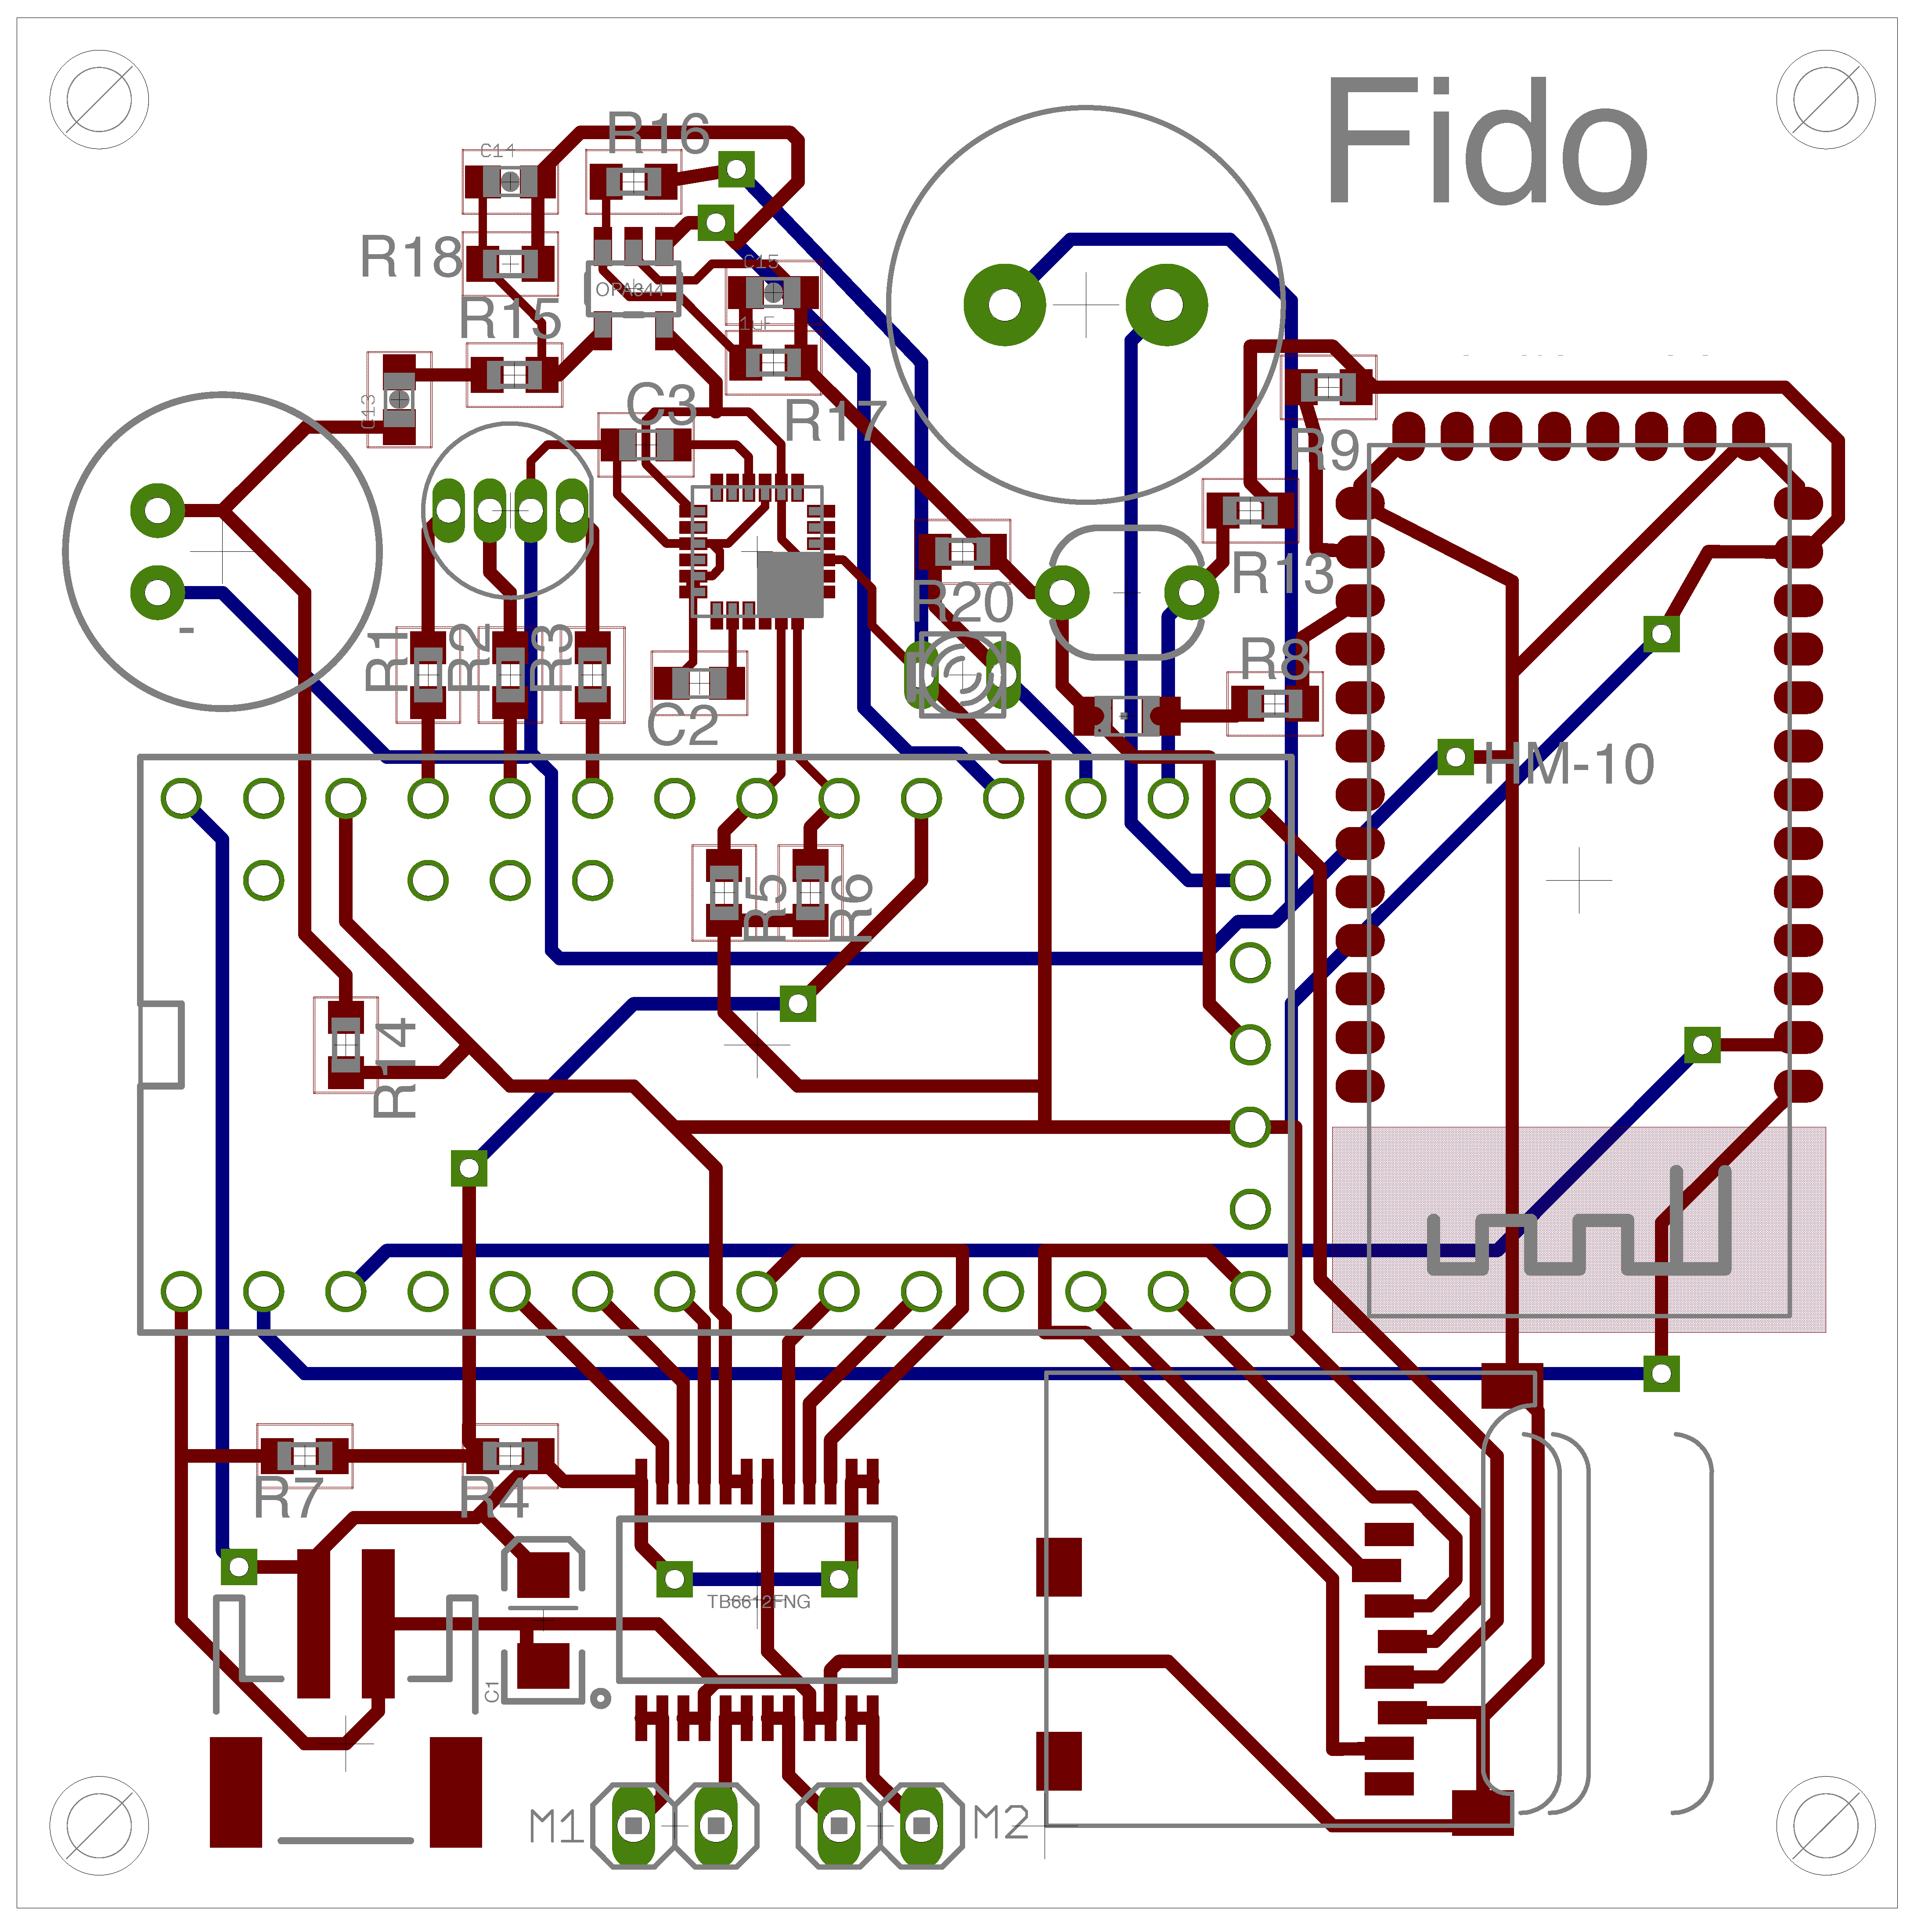
\includegraphics[height=5cm]{Figures/boardLayout.png}
	\caption{Fido PCB Layout}
\end{figure}

% cad render/screenshot

A printed circuit board was routed in CadSoft EAGLE based on the schematic described above, then manufactured by Smart Prototyping in Hong Kong.  The boards were hand assembled (somewhat painstakingly) including all 37 components using standard through-hole and surface-mount soldering techniques.  This included use of both a standard soldering pencil and a hot-air rework station with solder paste.  The robot chassis was 3D modeled using Autodesk AutoCAD Student, then printed in PLA plastic using a Makerbot Replicator.